\definecolor{pj}{HTML}{66A3FE}
\definecolor{amm}{HTML}{FFF28A}
\definecolor{an}{HTML}{52D3FA}
\definecolor{ver}{HTML}{6665FE}
\definecolor{pg}{HTML}{FF6766}
\definecolor{resp}{HTML}{FFB166}
\definecolor{pj}{HTML}{7FA8FF}

\section{Pianificazione}
\subsection{Modello adottato}
Dopo un'attenta valutazione e analisi delle esigenze del progetto, il team ha deciso di adottare un approccio di sviluppo iterativo e incrementale per la realizzazione del software richiesto. È stato quindi deciso di adoperare il modello \textit{Agile}, con particolare attenzione al framework \textit{Scrum}.\\
Avendo necessità di risposta efficace alle sfide e alle plurime esigenze dello sviluppo software, pensiamo che questo approccio sia il migliore.\\
Attraverso l'adozione dello Scrum, il team mira ad influenzare nel modo più significativo e positivo possibile il successo del progetto.

\subsection{Vantaggi adozione dello Scrum}
\begin{itemize}
    \item \textbf{Flessibilità e adattabilità}: il framework Scrum consente una rapida risposta ai cambiamenti nei requisiti del cliente, garantendo una maggiore flessibilità durante tutto il periodo di sviluppo;
    \item \textbf{collaborazione e comunicazione}: la struttura del framework incentiva una comunicazione aperta e continua tra i membri del team e le parti interessate, migliorando la comprensione reciproca, la condivisione di conoscenze e facilitando l'avanzamento dello sviluppo;
    \begin{itemize}
        \item In particolare con l’azienda proponente sono fissati \textit{SAL} (\textbf{S}tato \textbf{A}vanzamento \textbf{L}avori) ogni due settimane.
    \end{itemize}
    \item \textbf{consegna incrementale}: attraverso la pratica di rilasci incrementali, vi è la possibilità di una distribuzione graduale delle funzionalità. Questo permette al cliente di valutare il prodotto in anticipo e di fornire feedback tempestivi;
    \item \textbf{miglioramento continuo}: il framework Scrum promuove un approccio iterativo e incrementale allo sviluppo, consentendo al team di apprendere dagli errori e di apportare miglioramenti costanti al processo di sviluppo.
\end{itemize}
La scelta di adottare il framework Scrum riflette la nostra propensione a produrre e fornire un prodotto di qualità, in modo da garantire una risposta efficiente ed efficace alle possibili nuove richieste che il cliente potrebbe avanzare.

\subsection{Gestione e monitoraggio del progetto}
In accordo con l'azienda proponente, è stato deciso di organizzare l’avanzamento del progetto in periodi di durata prefissata seguendo un approccio simile agli sprint relativi al framework Scrum.
Durante ciascun periodo di sviluppo, verranno decisi gli obiettivi da raggiungere e le attività da svolgere, in accordo con l'azienda proponente e i membri del team. La scelta degli obiettivi e attività da portare a termine durante il periodo saranno scelte attraverso un'accurata analisi che comprenderà:
\begin{itemize}
    \item l'\textbf{importanza strategica} delle attività;
    \item la \textbf{fattibilità di completare le attività} entro la durata del periodo di riferimento.
\end{itemize}
Nel remoto caso in cui alcune attività non debbano essere portate a termine nei termini indicati, queste verranno riportate nel consuntivo di periodo e proseguiranno nel periodo successivo. Ogni periodo sarà documentato attraverso una tabella esaustiva in cui saranno identificate le task relative a ciascun ruolo. Per ogni attività verrà indicato lo stato di completamento, i tempi previsti ed effettivi, e i costi associati. Al termine di ciascun periodo, sarà calcolato il costo totale del progetto fino a quel momento, fornendo una chiara visione del progresso complessivo. Inoltre ogni periodo conterrà una discussione sui rischi occorsi e sull’esito della loro mitigazione seguendo quanto definito nella sezione apposita. I dati riportati per ciascun periodo rappresentano un riepilogo delle informazioni inserite durante la fase di pianificazione e di preventivazione da parte del responsabile, nonché delle registrazioni orarie effettuate autonomamente dai membri del team tramite un'apposita funzione di \href{https://7last.github.io/docs/rtb/documentazione-interna/glossario#clickup}{ClickUp\textsubscript{G}}.

\subsection{Periodi}
Per ogni periodo si riportano di seguito le seguenti informazioni:
\begin{itemize}
    \item data di inizio, data di fine prevista, data di fine attuale ed eventuali giorni di ritardo;
    \item pianificazione delle attività da svolgere al suo interno (avanzamento atteso), con tanto di potenziali rischi;
    \item tempo stimato per poter completare tutte le attività previste;
    \item confronto fra il lavoro svolto (avanzamento conseguito) e quello preventivato, con annessa analisi dei costi;
    \item rischi effettivamente occorsi, valutandone il loro impatto e la loro mitigazione;
    \item retrospettiva di periodo per capire cosa e come migliorare in futuro e cosa invece mantenere;
\end{itemize}
I periodi vengono suddivisi in 3 grandi insiemi corrispondenti alle revisioni di avanzamento del progetto:
\begin{itemize}
    \item \textbf{RTB}: \textit{\textbf{R}equirements and \textbf{T}echnology \textbf{B}aseline};
    \item \textbf{PB}:  \textit{\textbf{P}roduct \textbf{B}aseline};
    \item \textbf{CA}:  \textit{\textbf{C}ustomer \textbf{A}cceptance}.
\end{itemize}

\subsection{Requirements and Technology Baseline}
\subsubsection{Primo sprint:}
\begin{itemize}
    \item Inizio: 2024-04-03;
    \item Fine: 2024-04-19;
    \item Fine attuale: 2024-04-22;
    \item Giorni di ritardo: 3.
\end{itemize}

\subsubsubsection{Pianificazione}
Durante questo periodo, il team si concentra sul dedicare risorse significative allo sviluppo, alla standardizzazione e all'automazione dei processi, ove possibile. Nel primo incontro con l'azienda proponente vengono definiti gli obiettivi chiave da raggiungere entro il prossimo SAL del 19 aprile 2024. \\
In particolare, questi obiettivi comprendono:
\begin{itemize}
    \item simulazione di un sensore mediante codice \textbf{Python};
    \item integrazione con \textbf{Apache Kafka} utilizzando ambiente \textbf{Docker}.
\end{itemize}
Parallelamente a questa fase, l'amministratore ha stanziato risorse per automatizzare il processo di compilazione dei sorgenti LateX una volta caricati sul repository condiviso, e per distinguere automaticamente le parole presenti nel \href{https://7last.github.io/docs/rtb/documentazione-interna/glossario#glossario}{glossario\textsubscript{G}} da quelle che non lo sono.

\subsubsubsubsection{Rischi attesi}
I rischi attesi per questo periodo sono:
\begin{itemize}
    \item Imprecisione nella pianificazione delle attività (Rischio RO1);
    \item Elevati costi delle attività (Rischio RO3);
    \item Rischio di conflitti interni (Rischio RC1);
    \item Problemi di comunicazione (Rischio RC2);
    \item Inesperienza nell'uso delle tecnologie adottate (Rischio RT1).
\end{itemize}
Ciò è causato dal fatto che, poiché siamo ancora all'inizio del progetto, non abbiamo ancora una chiara idea di come organizzarci per ottimizzare l'uso del tempo e delle risorse.

\newpage
\subsubsubsection{Preventivo}
Ruoli coinvolti: Responsabile (Re), Amministratore (Am), Analista (An), Programmatore (Pg), Verificatore (Ve).
\begin{table}[!h]
    \centering
    \begin{tabular}{ | l | c | c | c | c | c | c | c | }
        \hline
        \textbf{} & \textbf{Re} & \textbf{Am} &\textbf{An} & \textbf{Pj} & \textbf{Pg} & \textbf{Ve} & \textbf{Totale per persona} \\
        \hline
        Baldo            &  -   &  -   &  -   &  -   &  7   &  -   &  7   \\
        Benetazzo        &  -   &  7.5 &  -   &  -   &  -   &  -   &  7.5 \\
        Ferro            &  -   &  -   &  -   &  -   & 10   &  -   & 10   \\
        Malgarise        &  -   &  -   &  7   &  -   &  -   &  -   &  7   \\
        Occhinegro       &  -   &  -   &  -   &  -   &  -   &  9   &  9   \\
        Seganfreddo      &  -   &  -   &  7   &  -   &  -   &  -   &  7   \\
        Tiozzo           &  7.5 &  -   &  -   &  -   &  -   &  -   &  7.5 \\
        \hline
        Totale per ruolo &  7.5 &  7.5 & 14   &  -   & 17   &  9   &  -   \\
        \hline
    \end{tabular}
    \caption{Preventivo orario per ruolo dei membri del team durante il primo sprint}
    \label{tab:13}
\end{table}

%---------1_ISTOGRAMMA-----------%
\begin{figure}[!h]
    \centering
    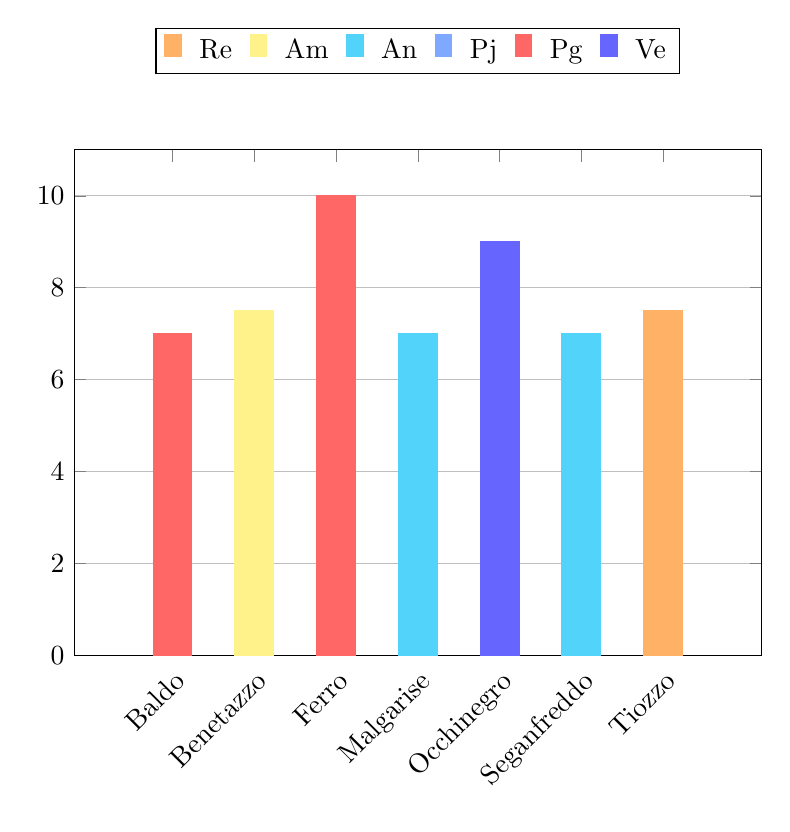
\begin{tikzpicture}
        \begin{axis}[
            width  = 0.85*\textwidth,
            height = 8cm,
            ybar stacked,
            bar width=14pt,
            ymajorgrids = true,
            symbolic x coords={Baldo, Benetazzo, Ferro, Malgarise, Occhinegro, Seganfreddo, Tiozzo},
            xtick = data,
            scaled y ticks = false,
            enlarge x limits=0.2,
            ymin=0,
            legend cell align=left,
            legend style={
                at={(0.5,1.15)},
                anchor=south,
                column sep=1ex,
                legend columns=-1
            },
            xticklabel style={rotate=45, anchor=north east, yshift=0ex, xshift=0ex},
            ]
            \addplot+[ybar, resp, fill=resp, mark=none] plot coordinates {
                (Baldo, 0)
                (Benetazzo, 0)
                (Ferro, 0)
                (Malgarise, 0)
                (Occhinegro, 0)
                (Seganfreddo, 0)
                (Tiozzo, 7.5)
            };
            \addplot+[ybar, amm, fill=amm, mark=none] plot coordinates {
                (Baldo, 0)
                (Benetazzo, 7.5)
                (Ferro, 0)
                (Malgarise, 0)
                (Occhinegro, 0)
                (Seganfreddo, 0)
                (Tiozzo, 0)
            };
            \addplot+[ybar, an, fill=an, mark=none] plot coordinates {
                (Baldo, 0)
                (Benetazzo, 0)
                (Ferro, 0)
                (Malgarise, 7)
                (Occhinegro, 0)
                (Seganfreddo, 7)
                (Tiozzo, 0)
            };
            \addplot+[ybar, pj, fill=pj, mark=none] plot coordinates {
                (Baldo, 0)
                (Benetazzo, 0)
                (Ferro, 0)
                (Malgarise, 0)
                (Occhinegro, 0)
                (Seganfreddo, 0)
                (Tiozzo, 0)
            };
            \addplot+[ybar, pg, fill=pg, mark=none] plot coordinates {
                (Baldo, 7)
                (Benetazzo, 0)
                (Ferro, 10)
                (Malgarise, 0)
                (Occhinegro, 0)
                (Seganfreddo, 0)
                (Tiozzo, 0)
            };
            \addplot+[ybar, ver, fill=ver, mark=none] plot coordinates {
                (Baldo, 0)
                (Benetazzo, 0)
                (Ferro, 0)
                (Malgarise, 0)
                (Occhinegro, 9)
                (Seganfreddo, 0)
                (Tiozzo, 0)
            };
        \legend{Re, Am, An, Pj, Pg, Ve}
        \end{axis}
    \end{tikzpicture}
    \caption{Impegno preventivo per ruolo dei membri del team durante il primo sprint}
    \label{fig:3}
\end{figure}

\newblock
%---------1_GRAFICO A TORTA-----------%
\begin{figure}[!h]
    \centering
    \begin{tikzpicture}
        \def\printonlypositive#1{\ifdim#1pt>0pt
        #1
        \fi}
        \pie[pos={8,0},radius=3.5,sum=auto,text=legend,
        before number=\printonlypositive,color={resp,amm,an,pj,pg,ver}] {
            14/Responsabile,
            14/Amministratore,
            25/Analista,
             0/Progettista,
            31/Programmatore,
            16/Verificatore
        }
        \end{tikzpicture}
    \caption{Ripartizione in percentuale dei ruoli nel primo sprint}
    \label{fig:4}
\end{figure}

\newpage
\subsubsubsection{Consuntivo}
Le attività previste sono state tutte svolte con successo. Abbiamo completato tutte le richieste della proponente con anticipo rispetto alla data di fine prevista.

\subsubsubsubsection{Prospetto orario}
\begin{table}[!h]
    \centering
    \begin{tabular}{ | l | c | c | c | c | c | c | c | }
        \hline
        \textbf{} & \textbf{Re} & \textbf{Am} & \textbf{An} & \textbf{Pj} & \textbf{Pg} & \textbf{Ve} & \textbf{Totale per persona} \\
        \hline
        Baldo            &  -   &  -   &  -   &  -   &  6   &  -   &  6   \\
        Benetazzo        &  -   &  6.5 &  -   &  -   &  -   &  -   &  6.5 \\
        Ferro            &  -   &  -   &  -   &  -   &  9   &  -   &  9   \\
        Malgarise        &  -   &  -   &  5   &  -   &  -   &  -   &  5   \\
        Occhinegro       &  -   &  -   &  -   &  -   &  -   &  9   &  9   \\
        Seganfreddo      &  -   &  -   &  5   &  -   &  -   &  -   &  5   \\
        Tiozzo           &  6.5 &  -   &  -   &  -   &  -   &  -   &  6.5 \\
        \hline
        Totale per ruolo &  6.5 &  6.5 & 10   &  0   & 15   &  9   &  -   \\
        \hline
    \end{tabular}
    \caption{Consuntivo orario per ruolo dei membri del team durante il primo sprint}
    \label{tab:14}
\end{table}

\subsubsubsubsection{Prospetto economico}
\begin{table}[!h]
    \centering
    \begin{tabular}{ | l | c | c | c | c | c | }
        \hline
        \textbf{Ruolo} & \textbf{Ore} & \textbf{Costo} & \textbf{Ore rimanenti preventivo} & \textbf{Ore rimanenti consuntivo} \\
        \hline
        Responsabile               &  6.5 &  195,00 € &  48.5 &  49.5 \\
        Amministratore             &  6.5 &  130,00 € &  48.5 &  49.5 \\
        Analista                   & 10   &  250,00 € &  64   &  68   \\
        Progettista                &  0   &    0,00 € & 112   & 112   \\
        Programmatore              & 15   &  225,00 € & 151   & 153   \\
        Verificatore               &  9   &  135,00 € & 165   & 165   \\
        \hline
        \textbf{Totale preventivo} & 55   & 1115,00 € & 589   &   -   \\
        \hline
        \textbf{Totale consuntivo} & 47   &  935,00 € &   -   & 597   \\
        \hline
    \end{tabular}
    \caption{Prospetto economico consuntivo durante il primo sprint}
    \label{tab:15}
\end{table}

\newpage
\subsubsubsubsection{Rischi effettivamente occorsi e loro mitigazione}
\begin{table}[!h]
    \centering
    \begin{tabular}{ | p{6cm} | p{2.5cm} | p{7.5cm} | }
        \hline
        \textbf{Tipologia} & \textbf{Rischio preventivato} & \textbf{Mitigazione}  \\
        \hline
        Inesperienza del team (Rischio \textbf{RT2}) & SI & Confronto con gli altri gruppi per la gestione dell'organizzazione.\\
        \hline
        Inesperienza nell'uso delle tecnologie adottate (Rischio \textbf{RT3}) & SI & Autoformazione e discussione interna e con la proponente.\\
        \hline
        Ritardi rispetto alle tempistiche previste (Rischio \textbf{RO3})& NO & Anticipati alcuni compiti previsti per il prossimo sprint.\\
        \hline
    \end{tabular}
    \caption{Rischi effettivamente occorsi e loro mitigazione durante il primo periodo}
    \label{tab:16}
\end{table}

\subsubsubsection{Retrospettiva}
La suddivisione iniziale dei ruoli per il presente sprint si è rivelata efficace e ben pensata. Ciascun componente ha lavorato senza essere sovraccaricato e il lavoro è stato distribuito in modo equo e senza disparità. \\
In seguito alla convocazione per il primo \textit{Diario di Bordo} avvenuta con scarso preavviso e prevista per data e ora in cui era stato pianificato il primo \textit{SAL} con l'azienda abbiamo dovuto posticipare al 22 aprile l'incontro con la proponente e questo ha causato un ritardo di 3 giorni inaspettato. Per rimediare a questo ritardo abbiamo iniziato ad effettuare dei progressi sulla documentazione previsti per lo sprint successivo. \\
Un'ulteriore problematica riscontrata è stata la difficoltà nell'adozione di alcune tecnologie, causando il rallentamento del lavoro. Per il prossimo sprint, si cercherà di risolvere questo problema con una maggiore formazione e con una maggiore collaborazione tra i membri del gruppo.

\newpage
\subsubsection{Secondo sprint:}
\begin{itemize}
    \item Inizio: 2024-04-23
    \item Fine: 2024-05-06
    \item Fine attuale: 2024-05-06
    \item Giorni di ritardo: nessuno.
\end{itemize}

\subsubsubsection{Pianificazione}
Durante il secondo periodo, il nostro team si propone di integrare \textit{Grafana} che rappresenta l'ultimo elemento dello stack tecnologico del Proof of Concept, come concordato nel corso del primo SAL. Inoltre, si prevede l'implementazione della funzionalità di visualizzazione tramite grafici delle misurazioni raccolte,
assieme ad una maggiore persistenza per quanto riguarda i dati raccolti all'interno di \textit{ClickHouse}. \\
Dal punto di vista della documentazione, invece, ci si pone l'obiettivo di portare a compimento il documento \textit{Norme di Progetto}, in modo da avere un quadro chiaro e definito delle regole e delle convenzioni da seguire durante lo sviluppo del progetto. In concomitanza con questa attività, si prosegue con la stesura del \textit{Piano di Progetto}, in particolare con la documentazione del primo e del secondo sprint, con l'aggiornamento continuo dei documenti \textit{Glossario} e \textit{Piano di Qualifica} e, infine, si può procedere con la stesura del documento \textit{Analisi dei Requisiti}, con lo scopo di identificare i casi d'uso fondamentali. \\
Per quanto riguarda gli strumenti adottati, il team prevede di assegnare risorse per l'analisi attenta della tecnologia proposta \textit{Redpanda} che andrebbe a sostituire \textit{Apache Kafka}, consigliata dalla proponente. Questa fase di valutazione mira a selezionare con attenzione le tecnologie più adatte al compimento delle specifiche del capitolato.

\subsubsubsubsection{Rischi attesi}
I rischi attesi per questo periodo sono:
\begin{itemize}
    \item Inesperienza nella pianificazione delle attività (Rischio RO1);
    \item Impegni personali o universitari (Rischio RO2);
    \item Inesperienza nell'uso delle tecnologie adottate (Rischio RT1);
    \item Problemi di compatibilità tra le tecnologie adottate (Rischio RT3);
    \item Rischio di conflitti interni (Rischio RC1).
\end{itemize}
Le differenze rispetto ai rischi attesi nel primo sprint non sono così significative, questo perchè l'esperienza del gruppo è ancora acerba e limitata.
A queste si aggiungono problematiche riguardo agli impegni personali, anche legati alle festività di questo periodo. Infine l'introduzione di \textit{Grafana},
tecnologia nuova all'interno del team, potrebbe causare problemi di ineseperienza e compatibilità con le tecnologie già adottate.

\subsubsubsection{Preventivo}
Ruoli coinvolti: Responsabile (Re), Amministratore (Am), Analista (An), Progettista (Pj), Programmatore (Pg), Verificatore (Ve).
\begin{table}[!h]
    \centering
    \begin{tabular}{ | l | c | c | c | c | c | c | c | }
        \hline
        \textbf{} & \textbf{Re} & \textbf{Am} &\textbf{An} & \textbf{Pj} & \textbf{Pg} & \textbf{Ve} & \textbf{Totale per persona} \\
        \hline
        Baldo            &  -   &  5   &  -   &  -   &  -   &  -   &  5   \\
        Benetazzo        &  -   &  -   &  -   &  -   &  -   &  7   &  7   \\
        Ferro            &  -   &  -   & 10   &  -   &  -   &  -   & 10   \\
        Malgarise        &  6   &  -   &  -   &  -   &  -   &  -   &  6   \\
        Occhinegro       &  -   &  -   &  -   &  -   & 10   &  -   & 10   \\
        Seganfreddo      &  -   &  -   &  -   &  7   &  -   &  -   &  7   \\
        Tiozzo           &  -   &  -   &  -   &  -   & 10   &  -   & 10   \\
        \hline
        Totale per ruolo &  6   &  5   & 10   &  7   & 20   &  7   &  -   \\
        \hline
    \end{tabular}
    \caption{Preventivo orario per ruolo dei membri del team durante il secondo sprint}
    \label{tab:17}
\end{table}

\newpage
%---------1_ISTOGRAMMA-----------%
\begin{figure}[!h]
    \centering
    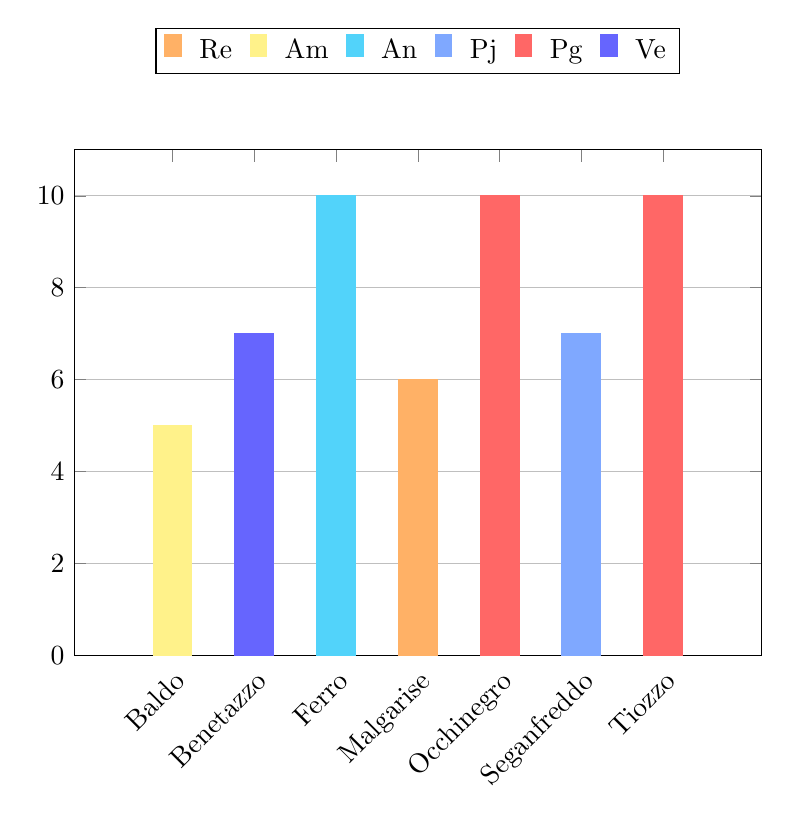
\begin{tikzpicture}
        \begin{axis}[
            width  = 0.85*\textwidth,
            height = 8cm,
            ybar stacked,
            bar width=14pt,
            ymajorgrids = true,
            symbolic x coords={Baldo, Benetazzo, Ferro, Malgarise, Occhinegro, Seganfreddo, Tiozzo},
            xtick = data,
            scaled y ticks = false,
            enlarge x limits=0.2,
            ymin=0,
            legend cell align=left,
            legend style={
                at={(0.5,1.15)},
                anchor=south,
                column sep=1ex,
                legend columns=-1
            },
            xticklabel style={rotate=45, anchor=north east, yshift=0ex, xshift=0ex},
            ]
            \addplot+[ybar, resp, fill=resp, mark=none] plot coordinates {
                (Baldo, 0)
                (Benetazzo, 0)
                (Ferro, 0)
                (Malgarise, 6)
                (Occhinegro, 0)
                (Seganfreddo, 0)
                (Tiozzo, 0)
            };
            \addplot+[ybar, amm, fill=amm, mark=none] plot coordinates {
                (Baldo, 5)
                (Benetazzo, 0)
                (Ferro, 0)
                (Malgarise, 0)
                (Occhinegro, 0)
                (Seganfreddo, 0)
                (Tiozzo, 0)
            };
            \addplot+[ybar, an, fill=an, mark=none] plot coordinates {
                (Baldo, 0)
                (Benetazzo, 0)
                (Ferro, 10)
                (Malgarise, 0)
                (Occhinegro, 0)
                (Seganfreddo, 0)
                (Tiozzo, 0)
            };
            \addplot+[ybar, pj, fill=pj, mark=none] plot coordinates {
                (Baldo, 0)
                (Benetazzo, 0)
                (Ferro, 0)
                (Malgarise, 0)
                (Occhinegro, 0)
                (Seganfreddo, 7)
                (Tiozzo, 0)
            };
            \addplot+[ybar, pg, fill=pg, mark=none] plot coordinates {
                (Baldo, 0)
                (Benetazzo, 0)
                (Ferro, 0)
                (Malgarise, 0)
                (Occhinegro, 10)
                (Seganfreddo, 0)
                (Tiozzo, 10)
            };
            \addplot+[ybar, ver, fill=ver, mark=none] plot coordinates {
                (Baldo, 0)
                (Benetazzo, 7)
                (Ferro, 0)
                (Malgarise, 0)
                (Occhinegro, 0)
                (Seganfreddo, 0)
                (Tiozzo, 0)
            };
            \legend{Re, Am, An, Pj, Pg, Ve}
        \end{axis}
    \end{tikzpicture}
    \caption{Impegno preventivo per ruolo dei membri del team durante il secondo sprint}
    \label{fig:5}
\end{figure}

%---------1_GRAFICO A TORTA-----------%
\begin{figure}[!h]
    \centering
    \begin{tikzpicture}
        \def\printonlypositive#1{\ifdim#1pt>0pt
        #1
        \fi}
        \pie[pos={8,0},radius=3.5,sum=auto,text=legend,
        before number=\printonlypositive,color={resp,amm,an,pj,pg,ver}] {
            11/Responsabile,
             9/Amministratore,
            18/Analista,
            13/Progettista,
            36/Programmatore,
            13/Verificatore
        }
        \end{tikzpicture}
    \caption{Ripartizione in percentuale dei ruoli nel secondo sprint}
    \label{fig:6}
\end{figure}

\newpage
\subsubsubsection{Consuntivo}
Tutte le attività previste sono state svolte con successo. Come si può notare dal prospetto orario, i Programmatori hanno richiesto più ore rispetto a quanto preventivato, al contrario, l'Analista ha richiesto meno ore.

\subsubsubsubsection{Prospetto orario}
\begin{table}[!h]
    \centering
    \begin{tabular}{ | l | c | c | c | c | c | c | c | }
        \hline
        \textbf{} & \textbf{Re} & \textbf{Am} &\textbf{An} & \textbf{Pj} & \textbf{Pg} & \textbf{Ve} & \textbf{Totale per persona} \\
        \hline
        Baldo            &  -   &  5   &  -   &  -   &  -   &  -   &  5   \\
        Benetazzo        &  -   &  -   &  -   &  -   &  -   &  6   &  6   \\
        Ferro            &  -   &  -   & 10   &  -   &  -   &  -   & 10   \\
        Malgarise        &  6   &  -   &  -   &  -   &  -   &  -   &  6   \\
        Occhinegro       &  -   &  -   &  -   &  -   &  9   &  -   &  9   \\
        Seganfreddo      &  -   &  -   &  -   &  7   &  -   &  -   &  7   \\
        Tiozzo           &  -   &  -   &  -   &  -   &  9   &  -   &  9   \\
        \hline
        Totale per ruolo &  6   &  5   & 10   &  7   & 18   &  6   &  -   \\
        \hline
    \end{tabular}
    \caption{Consuntivo orario per ruolo dei membri del team durante il secondo sprint}
    \label{tab:18}
\end{table}

\subsubsubsubsection{Prospetto economico}
\begin{table}[!h]
    \centering
    \begin{tabular}{ | l | c | c | c | c | c | }
        \hline
        \textbf{Ruolo} & \textbf{Ore} & \textbf{Costo} & \textbf{Ore rimanenti preventivo} & \textbf{Ore rimanenti consuntivo} \\
        \hline
        Responsabile               &  6   &  180,00 € &  43.5 &  43.5 \\
        Amministratore             &  5   &  100,00 € &  44.5 &  44.5 \\
        Analista                   & 10   &  250,00 € &  58   &  58   \\
        Progettista                &  7   &  175,00 € & 105   & 105   \\
        Programmatore              & 18   &  270,00 € & 133   & 135   \\
        Verificatore               &  6   &   90,00 € & 158   & 159   \\
        \hline
        \textbf{Totale preventivo} & 55   & 1110,00 € & 542   &   -   \\
        \hline
        \textbf{Totale consuntivo} & 52   & 1065,00 € &   -   & 545   \\
        \hline
    \end{tabular}
    \caption{Consuntivo economico consuntivo durante il secondo sprint}
    \label{tab:19}
\end{table}

\subsubsubsubsection{Rischi effettivamente occorsi e loro mitigazione}
\begin{table}[!h]
    \centering
    \begin{tabular}{ | p{6cm} | p{2.5cm} | p{7.5cm} | }
        \hline
        \textbf{Tipologia} & \textbf{Rischio preventivato} & \textbf{Mitigazione}  \\
        \hline
        Inesperienza del team (Rischio \textbf{RO1}) & SI & Ridistribuzione compiti assegnati durante lo sprint.\\
        \hline
        Impegni personali o universitari (Rischio \textbf{RO2})& NO & Comunicato in anticipo gli impegni, lavoro affidato svolto prima o dopo l'impegno.\\
        \hline
        Inesperienza nell'uso delle tecnologie adottate (Rischio \textbf{RT3}) & SI & Autoformazione e pair programming.\\
        \hline
    \end{tabular}
    \caption{Rischi effettivamente occorsi e loro mitigazione durante il primo periodo}
    \label{tab:20}
\end{table}

\subsubsubsection{Retrospettiva}
La suddivisione dei compiti da svolgere non è stata ottimale, in quanto alcuni membri del team hanno completato le attività assegnate in anticipo rispetto alla data di fine prevista, mentre altri hanno richiesto più tempo del previsto. Per i prossimi sprint valuteremo soluzioni alternative per evitare che ciò accada nuovamente. \\
Alcuni membri del gruppo hanno avuto impegni personali imprevisti durante questo periodo che hanno portato via del tempo prezioso per il completamento delle attività previste. Tali impegni sono stati comunicati tempestivamente al team e i compiti assegnati sono stati completati prima o dopo l'impegno. \\
Permane la difficoltà nell'uso delle tecnologie previste. In seguito alla turnazione dei ruoli altri membri del team si sono ritrovati a dover affrontare le stesse difficoltà avute dai colleghi in precedenza. In questo caso le difficoltà avute sono state superate mediante attività di autoformazione e \textit{pair programming} assieme ai compagni che avevano risolto gli stessi problemi nello sprint precedente.

\newpage
\subsubsection{Terzo sprint:}
\begin{itemize}
    \item Inizio: 2024-05-07
    \item Fine: 2024-05-15
    \item Fine attuale: 2024-05-15
    \item Giorni di ritardo: nessuno.
\end{itemize}

\subsubsubsection{Pianificazione}
In questo periodo il gruppo si concentrerà ad analizzare le possibilità di miglioramento suggerite dallàzienda per quanto riguarda la visualizzazione dei dati in \textit{Grafana}. Molte risorse saranno ancora dedicate alla documentazione, in particolare al documento \textit{Analisi dei Requisiti} e al \textit{Piano di Progetto}. \\
Durante il \textit{SAL} del precedente sprint sono stati fissati con l'azienda i seguenti obiettivi:
\begin{itemize}
    \item correzione della visualizzazione di latitudine e longitudine (con tutti i decimali);
    \item aggiunta di filtri per migliorare la visualizzazione dei dati, anche per poter visualizzare quelli di un singolo sensore;
    \item rendere più chiaro il grafico \textit{Daily mean};
    \item togliere il grafico \textit{Average temperature per minute} o sostituirlo con un grafico più significativo;
    \item raffinamento globale della dashboard.
\end{itemize}

\subsubsubsubsection{Rischi attesi}
I rischi attesi per questo periodo sono:
\begin{itemize}
    \item Inesperienza del team nella pianificazione delle attività (Rischio RO1);
    \item Ritardi rispetto alle tempistiche previste (Rischio RO3);
    \item Inesperienza nell'uso delle tecnologie adottate (Rischio RT1).
\end{itemize}
Siamo ancora nelle fasi iniziali del progetto, dobbiamo ancora imparare come pianificare le attività al meglio; inoltre molti membri del gruppo non hanno mai usato le tecnologie previste.

\subsubsubsection{Preventivo}
Ruoli coinvolti: Responsabile (Re), Amministratore (Am), Analista (An), Progettista (Pj), Programmatore (Pg), Verificatore (Ve).
\begin{table}[!h]
    \centering
    \begin{tabular}{ | l | c | c | c | c | c | c | c | }
        \hline
        \textbf{} & \textbf{Re} & \textbf{Am} &\textbf{An} & \textbf{Pj} & \textbf{Pg} & \textbf{Ve} & \textbf{Totale per persona} \\
        \hline
        Baldo            &  -   &  -   &  -   &  -   &  -   &  4   &  4   \\
        Benetazzo        &  4   &  -   &  -   &  -   &  -   &  -   &  4   \\
        Ferro            &  -   &  -   &  -   &  5   &  -   &  -   &  5   \\
        Malgarise        &  -   &  -   &  -   &  -   &  5   &  -   &  5   \\
        Occhinegro       &  -   &  -   &  6   &  -   &  -   &  -   &  6   \\
        Seganfreddo      &  -   &  -   &  -   &  -   &  5   &  -   &  5   \\
        Tiozzo           &  -   &  5   &  -   &  -   &  -   &  -   &  5   \\
        \hline
        Totale per ruolo &  4   &  5   &  6   &  5   & 10   &  4   &  -   \\
        \hline
    \end{tabular}
    \caption{Preventivo orario per ruolo dei membri del team durante il terzo sprint}
    \label{tab:21}
\end{table}

%---------1_ISTOGRAMMA-----------%
\begin{figure}[!h]
    \centering
    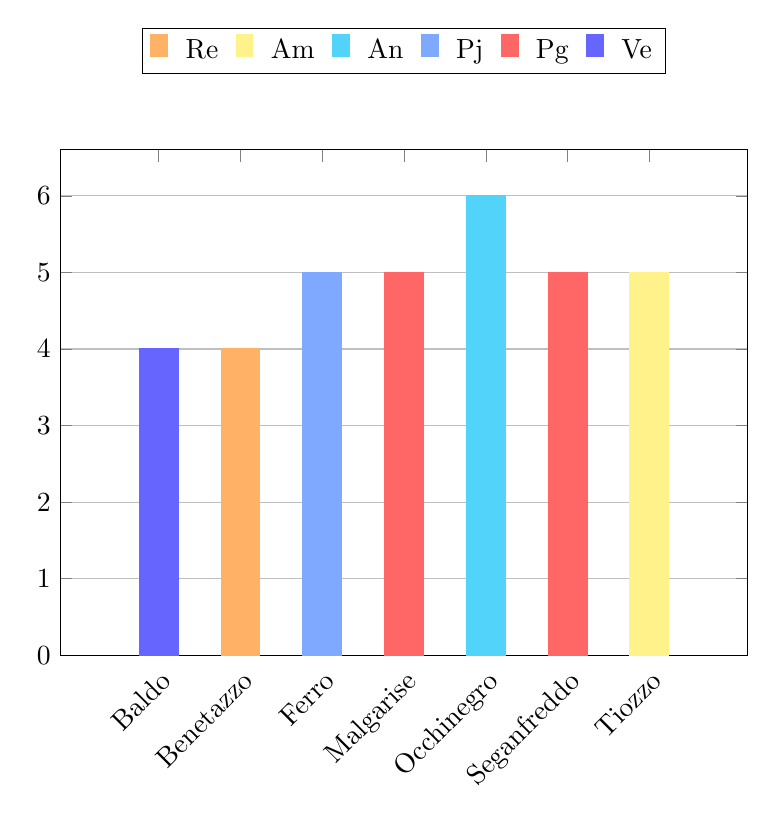
\begin{tikzpicture}
        \begin{axis}[
            width  = 0.85*\textwidth,
            height = 8cm,
            ybar stacked,
            bar width=14pt,
            ymajorgrids = true,
            symbolic x coords={Baldo, Benetazzo, Ferro, Malgarise, Occhinegro, Seganfreddo, Tiozzo},
            xtick = data,
            scaled y ticks = false,
            enlarge x limits=0.2,
            ymin=0,
            legend cell align=left,
            legend style={
                at={(0.5,1.15)},
                anchor=south,
                column sep=1ex,
                legend columns=-1
            },
            xticklabel style={rotate=45, anchor=north east, yshift=0ex, xshift=0ex},
            ]
            \addplot+[ybar, resp, fill=resp, mark=none] plot coordinates {
                (Baldo, 0)
                (Benetazzo, 4)
                (Ferro, 0)
                (Malgarise, 0)
                (Occhinegro, 0)
                (Seganfreddo, 0)
                (Tiozzo, 0)
            };
            \addplot+[ybar, amm, fill=amm, mark=none] plot coordinates {
                (Baldo, 0)
                (Benetazzo, 0)
                (Ferro, 0)
                (Malgarise, 0)
                (Occhinegro, 0)
                (Seganfreddo, 0)
                (Tiozzo, 5)
            };
            \addplot+[ybar, an, fill=an, mark=none] plot coordinates {
                (Baldo, 0)
                (Benetazzo, 0)
                (Ferro, 0)
                (Malgarise, 0)
                (Occhinegro, 6)
                (Seganfreddo, 0)
                (Tiozzo, 0)
            };
            \addplot+[ybar, pj, fill=pj, mark=none] plot coordinates {
                (Baldo, 0)
                (Benetazzo, 0)
                (Ferro, 5)
                (Malgarise, 0)
                (Occhinegro, 0)
                (Seganfreddo, 0)
                (Tiozzo, 0)
            };
            \addplot+[ybar, pg, fill=pg, mark=none] plot coordinates {
                (Baldo, 0)
                (Benetazzo, 0)
                (Ferro, 0)
                (Malgarise, 5)
                (Occhinegro, 0)
                (Seganfreddo, 5)
                (Tiozzo, 0)
            };
            \addplot+[ybar, ver, fill=ver, mark=none] plot coordinates {
                (Baldo, 4)
                (Benetazzo, 0)
                (Ferro, 0)
                (Malgarise, 0)
                (Occhinegro, 0)
                (Seganfreddo, 0)
                (Tiozzo, 0)
            };
        \legend{Re, Am, An, Pj, Pg, Ve}
        \end{axis}
    \end{tikzpicture}
    \caption{Impegno preventivo per ruolo dei membri del team durante il terzo sprint}
    \label{fig:7}
\end{figure}

\newblock
%---------1_GRAFICO A TORTA-----------%
\begin{figure}[!h]
    \centering
    \begin{tikzpicture}
        \def\printonlypositive#1{\ifdim#1pt>0pt
        #1
        \fi}
        \pie[pos={8,0},radius=3.5,sum=auto,text=legend,
        before number=\printonlypositive,color={resp,amm,an,pj,pg,ver}] {
            12/Responsabile,
            15/Amministratore,
            18/Analista,
            15/Progettista,
            29/Programmatore,
            12/Verificatore
        }
        \end{tikzpicture}
    \caption{Ripartizione in percentuale dei ruoli nel terzo sprint}
    \label{fig:8}
\end{figure}

\subsubsubsection{Consuntivo}
Anche per questo sprint, nonostante la durata ridotta, siamo riusciti a portare a termine tutte le attività previste.

\subsubsubsubsection{Prospetto orario}
\begin{table}[!h]
    \centering
    \begin{tabular}{ | l | c | c | c | c | c | c | c | }
        \hline
        \textbf{} & \textbf{Re} & \textbf{Am} & \textbf{An} & \textbf{Pj} & \textbf{Pg} & \textbf{Ve} & \textbf{Totale per persona} \\
        \hline
        Baldo            &  -   &  -   &  -   &  -   &  -   &  3   &  3   \\
        Benetazzo        &  4,5 &  -   &  -   &  -   &  -   &  -   &  4.5 \\
        Ferro            &  -   &  -   &  -   &  4   &  -   &  -   &  4   \\
        Malgarise        &  -   &  -   &  -   &  -   &  6   &  -   &  6   \\
        Occhinegro       &  -   &  -   &  5   &  -   &  -   &  -   &  5   \\
        Seganfreddo      &  -   &  -   &  -   &  -   &  6   &  -   &  6   \\
        Tiozzo           &  -   &  5.5 &  -   &  -   &  -   &  -   &  5.5 \\
        \hline
        Totale per ruolo &  4.5 &  5.5 &  5   &  4   & 12   &  3   &  -   \\
        \hline
    \end{tabular}
    \caption{Consuntivo orario per ruolo dei membri del team durante il terzo sprint}
    \label{tab:22}
\end{table}

\subsubsubsubsection{Prospetto economico}
\begin{table}[!h]
    \centering
    \begin{tabular}{ | l | c | c | c | c | c | }
        \hline
        \textbf{Ruolo} & \textbf{Ore} & \textbf{Costo} & \textbf{Ore rimanenti preventivo} & \textbf{Ore rimanenti consuntivo} \\
        \hline
        Responsabile               &  4.5 &  135,00 € &  39.5 &  39   \\
        Amministratore             &  5.5 &  110,00 € &  39.5 &  39   \\
        Analista                   &  5   &  125,00 € &  52   &  53   \\
        Progettista                &  4   &  100,00 € & 100   & 101   \\
        Programmatore              & 12   &  180,00 € & 125   & 123   \\
        Verificatore               &  3   &   45,00 € & 155   & 156   \\
        \hline
        \textbf{Totale preventivo} & 34   &  705,00 € & 511   &   -   \\
        \hline
        \textbf{Totale consuntivo} & 34   &  695,00 € &   -   & 511   \\
        \hline
    \end{tabular}
    \caption{Prospetto economico consuntivo durante il terzo sprint}
    \label{tab:23}
\end{table}

\subsubsubsubsection{Rischi effettivamente occorsi e loro mitigazione}
\begin{table}[!h]
    \centering
    \begin{tabular}{ | p{6cm} | p{2.5cm} | p{7.5cm} | }
        \hline
        \textbf{Tipologia} & \textbf{Rischio preventivato} & \textbf{Mitigazione}  \\
        \hline
        Inesperienza nell'uso delle tecnologie adottate (Rischio \textbf{RT3}) & SI & Autoformazione e pair programming.\\
        \hline
    \end{tabular}
    \caption{Rischi effettivamente occorsi e loro mitigazione durante il primo periodo}
    \label{tab:24}
\end{table}

\subsubsubsection{Retrospettiva}
Durante l'ultimo \textit{SAL} con l'azienda abbiamo deciso su loro consiglio di accorciare gli sprint, passando dalla durata di due settimane a quella di una settimana. Abbiamo anche deciso di spostare i prossimi al mercoledì, in quanto uno dei membri del gruppo era impossibilitato a partecipare il lunedì per impegni di lavoro. Questo ci ha permesso di avere due giorni in più in questo sprint e di attenuare l'impatto del cambiamento di durata. Questo, assieme ad un'attenta pianificazione delle attività, ci ha permesso di completare tutte le attività previste senza alcun ritardo e di prendere maggior confidenza con sprint di durata inferiore. \\
Permane la difficoltà nell'uso delle tecnologie adottate. In particolare abbiamo riscontrato in questo sprint diverse difficoltà nella configurazione di tali strumenti in diversi sistemi operativi. Come già sperimentato nel precedente sprint le attività di autoformazione e \textit{pair programming} si sono rivelate molto utili per superare tali difficoltà ed evitare ritardi nel completamento delle attività.

%--------- MODELLO X SPRINT SUCCESSIVI (occhio ai TODO) -----------%
% \newpage
% \subsubsection{Secondo sprint:} % TODO mettere numero di sprint corretto
% \begin{itemize}
%     \item Inizio: 2024-04-23 % TODO mettere data inizio corretta
%     \item Fine: 2024-05-06 % TODO mettere data fine corretta
%     \item Fine attuale: 2024-05-06 % TODO mettere data fine attuale corretta
%     \item Giorni di ritardo: nessuno. % TODO mettere giorni di ritardo corretti
% \end{itemize}
%
% \subsubsubsection{Pianificazione}
%  % TODO scrivere qualcosa sulla pianificazione dello sprint
%
% \subsubsubsubsection{Rischi attesi} % TODO mettere rischi attesi corretti nella lista
% I rischi attesi per questo periodo sono:
% \begin{itemize}
%     \item Inesperienza nella pianificazione delle attività (Rischio RO1);
%     \item Impegni personali o universitari (Rischio RO2);
%     \item Inesperienza nell'uso delle tecnologie adottate (Rischio RT1);
%     \item Problemi di compatibilità tra le tecnologie adottate (Rischio RT3);
%     \item Rischio di conflitti interni (Rischio RC1).
% \end{itemize}
%  % TODO commentare e motivare rischi attesi rispetto agli sprint precedenti
%
% \subsubsubsection{Preventivo} % TODO mettere valori corretti
% Ruoli coinvolti: Responsabile (Re), Amministratore (Am), Analista (An), Progettista (Pj), Programmatore (Pg), Verificatore (Ve).
% \begin{table}[!h]
%     \centering
%     \begin{tabular}{ | l | c | c | c | c | c | c | c | }
%         \hline
%         \textbf{} & \textbf{Re} & \textbf{Am} &\textbf{An} & \textbf{Pj} & \textbf{Pg} & \textbf{Ve} & \textbf{Totale per persona} \\
%         \hline
%         Baldo            &  -   &  -   &  -   &  -   &  -   &  -   &  -   \\
%         Benetazzo        &  -   &  -   &  -   &  -   &  -   &  -   &  -   \\
%         Ferro            &  -   &  -   &  -   &  -   &  -   &  -   &  -   \\
%         Malgarise        &  -   &  -   &  -   &  -   &  -   &  -   &  -   \\
%         Occhinegro       &  -   &  -   &  -   &  -   &  -   &  -   &  -   \\
%         Seganfreddo      &  -   &  -   &  -   &  -   &  -   &  -   &  -   \\
%         Tiozzo           &  -   &  -   &  -   &  -   &  -   &  -   &  -   \\
%         \hline
%         Totale per ruolo &  -   &  -   &  -   &  -   &  -   &  -   &  -   \\
%         \hline
%     \end{tabular}
%     \caption{Preventivo orario per ruolo dei membri del team durante il secondo sprint} % TODO mettere numero di sprint corretto
%     \label{tab:5} % TODO mettere numero di tabella corretto
% \end{table}
%
% \newpage
% %---------1_ISTOGRAMMA-----------%
% \begin{figure}[!h]
%     \centering
%     \begin{tikzpicture}
%         \begin{axis}[
%             width  = 0.85*\textwidth,
%             height = 8cm,
%             ybar stacked,
%             bar width=14pt,
%             ymajorgrids = true,
%             symbolic x coords={Baldo, Benetazzo, Ferro, Malgarise, Occhinegro, Seganfreddo, Tiozzo},
%             xtick = data,
%             scaled y ticks = false,
%             enlarge x limits=0.2,
%             ymin=0,
%             legend cell align=left,
%             legend style={
%                 at={(0.5,1.15)},
%                 anchor=south,
%                 column sep=1ex,
%                 legend columns=-1
%             },
%             xticklabel style={rotate=45, anchor=north east, yshift=0ex, xshift=0ex},
%             ] % TODO mettere valori corretti
%             \addplot+[ybar, resp, fill=resp, mark=none] plot coordinates {
%                 (Baldo, 0)
%                 (Benetazzo, 0)
%                 (Ferro, 0)
%                 (Malgarise, 0)
%                 (Occhinegro, 0)
%                 (Seganfreddo, 0)
%                 (Tiozzo, 0)
%             };
%             \addplot+[ybar, amm, fill=amm, mark=none] plot coordinates {
%                 (Baldo, 0)
%                 (Benetazzo, 0)
%                 (Ferro, 0)
%                 (Malgarise, 0)
%                 (Occhinegro, 0)
%                 (Seganfreddo, 0)
%                 (Tiozzo, 0)
%             };
%             \addplot+[ybar, an, fill=an, mark=none] plot coordinates {
%                 (Baldo, 0)
%                 (Benetazzo, 0)
%                 (Ferro, 0)
%                 (Malgarise, 0)
%                 (Occhinegro, 0)
%                 (Seganfreddo, 0)
%                 (Tiozzo, 0)
%             };
%             \addplot+[ybar, pj, fill=pj, mark=none] plot coordinates {
%                 (Baldo, 0)
%                 (Benetazzo, 0)
%                 (Ferro, 0)
%                 (Malgarise, 0)
%                 (Occhinegro, 0)
%                 (Seganfreddo, 0)
%                 (Tiozzo, 0)
%             };
%             \addplot+[ybar, pg, fill=pg, mark=none] plot coordinates {
%                 (Baldo, 0)
%                 (Benetazzo, 0)
%                 (Ferro, 0)
%                 (Malgarise, 0)
%                 (Occhinegro, 0)
%                 (Seganfreddo, 0)
%                 (Tiozzo, 0)
%             };
%             \addplot+[ybar, ver, fill=ver, mark=none] plot coordinates {
%                 (Baldo, 0)
%                 (Benetazzo, 0)
%                 (Ferro, 0)
%                 (Malgarise, 0)
%                 (Occhinegro, 0)
%                 (Seganfreddo, 0)
%                 (Tiozzo, 0)
%             };
%             \legend{Re, Am, An, Pj, Pg, Ve}
%         \end{axis}
%     \end{tikzpicture}
%     \caption{Impegno preventivo per ruolo dei membri del team durante il secondo sprint} % TODO mettere numero sprint corretto
%     \label{fig:3} % TODO mettere numero di figura corretto
% \end{figure}
%
% %---------1_GRAFICO A TORTA-----------%
% \begin{figure}[!h]
%     \centering
%     \begin{tikzpicture}
%         \def\printonlypositive#1{\ifdim#1pt>0pt
%         #1
%         \fi}
%         \pie[pos={8,0},radius=3.5,sum=auto,text=legend,
%         before number=\printonlypositive,color={resp,amm,an,pj,pg,ver}] { % TODO mettere valori corretti
%              0/Responsabile,
%              0/Amministratore,
%              0/Analista,
%              0/Progettista,
%              0/Programmatore,
%              0/Verificatore
%         }
%         \end{tikzpicture}
%     \caption{Ripartizione in percentuale dei ruoli nel secondo sprint} % TODO mettere numero sprint corretto
%     \label{fig:4} % TODO mettere numero di figura corretto
% \end{figure}
%
% \newpage
% \subsubsubsection{Consuntivo}
%  % TODO breve commento sull’andamento dello sprint
%
% \subsubsubsubsection{Prospetto orario} % TODO mettere valori corretti
% \begin{table}[!h]
%     \centering
%     \begin{tabular}{ | l | c | c | c | c | c | c | c | }
%         \hline
%         \textbf{} & \textbf{Re} & \textbf{Am} &\textbf{An} & \textbf{Pj} & \textbf{Pg} & \textbf{Ve} & \textbf{Totale per persona} \\
%         \hline
%         Baldo            &  -   &  -   &  -   &  -   &  -   &  -   &  -   \\
%         Benetazzo        &  -   &  -   &  -   &  -   &  -   &  -   &  -   \\
%         Ferro            &  -   &  -   &  -   &  -   &  -   &  -   &  -   \\
%         Malgarise        &  -   &  -   &  -   &  -   &  -   &  -   &  -   \\
%         Occhinegro       &  -   &  -   &  -   &  -   &  -   &  -   &  -   \\
%         Seganfreddo      &  -   &  -   &  -   &  -   &  -   &  -   &  -   \\
%         Tiozzo           &  -   &  -   &  -   &  -   &  -   &  -   &  -   \\
%         \hline
%         Totale per ruolo &  -   &  -   &  -   &  -   &  -   &  -   &  -   \\
%         \hline
%     \end{tabular}
%     \caption{Consuntivo orario per ruolo dei membri del team durante il secondo sprint} % TODO mettere numero sprint corretto
%     \label{tab:6} % TODO mettere numero di tabella corretto
% \end{table}
%
% \subsubsubsubsection{Prospetto economico} % TODO mettere valori corretti
% \begin{table}[!h]
%     \centering
%     \begin{tabular}{ | l | c | c | c | c | c | }
%         \hline
%         \textbf{Ruolo} & \textbf{Ore} & \textbf{Costo} & \textbf{Ore rimanenti preventivo} & \textbf{Ore rimanenti consuntivo} \\
%         \hline
%         Responsabile               &  0   &    0,00 € &   0   &   0   \\
%         Amministratore             &  0   &    0,00 € &   0   &   0   \\
%         Analista                   &  0   &    0,00 € &   0   &   0   \\
%         Progettista                &  0   &    0,00 € &   0   &   0   \\
%         Programmatore              &  0   &    0,00 € &   0   &   0   \\
%         Verificatore               &  0   &    0,00 € &   0   &   0   \\
%         \hline
%         \textbf{Totale preventivo} &  0   &    0,00 € &   0   &   -   \\
%         \hline
%         \textbf{Totale consuntivo} &  0   &    0,00 € &   -   &   0   \\
%         \hline
%     \end{tabular}
%     \caption{Consuntivo economico consuntivo durante il secondo sprint} % TODO mettere numero sprint corretto
%     \label{tab:7} % TODO mettere numero di tabella corretto
% \end{table}
%
% \subsubsubsubsection{Rischi effettivamente occorsi e loro mitigazione} % TODO mettere rischi occorsi corretti
% \begin{table}[!h]
%     \centering
%     \begin{tabular}{ | p{6cm} | p{2.5cm} | p{7.5cm} | }
%         \hline
%         \textbf{Tipologia} & \textbf{Rischio preventivato} & \textbf{Mitigazione}  \\
%         \hline
%         Inesperienza del team (Rischio \textbf{RO1}) & SI & Ridistribuzione compiti assegnati durante lo sprint.\\
%         \hline
%         Impegni personali o universitari (Rischio \textbf{RO2})& NO & Comunicato in anticipo % gli impegni, lavoro affidato svolto prima o dopo l'impegno.\\
%         \hline
%         Inesperienza nell'uso delle tecnologie adottate (Rischio \textbf{RT3}) & SI & Autoformazione e pair programming.\\
%         \hline
%     \end{tabular}
%     \caption{Rischi effettivamente occorsi e loro mitigazione durante il primo periodo}
%     \label{tab:4} % TODO mettere numero di tabella corretto
% \end{table}
%
% \subsubsubsection{Retrospettiva}
%  % TODO fare retrospettiva commentando rischi preventivati vs rischi occorsi e quanto fatto per mitigarli.
% 